\section{Stable Diffusion}
\label{sec:stable_diffusion}


\begin{figure}
    \centering
    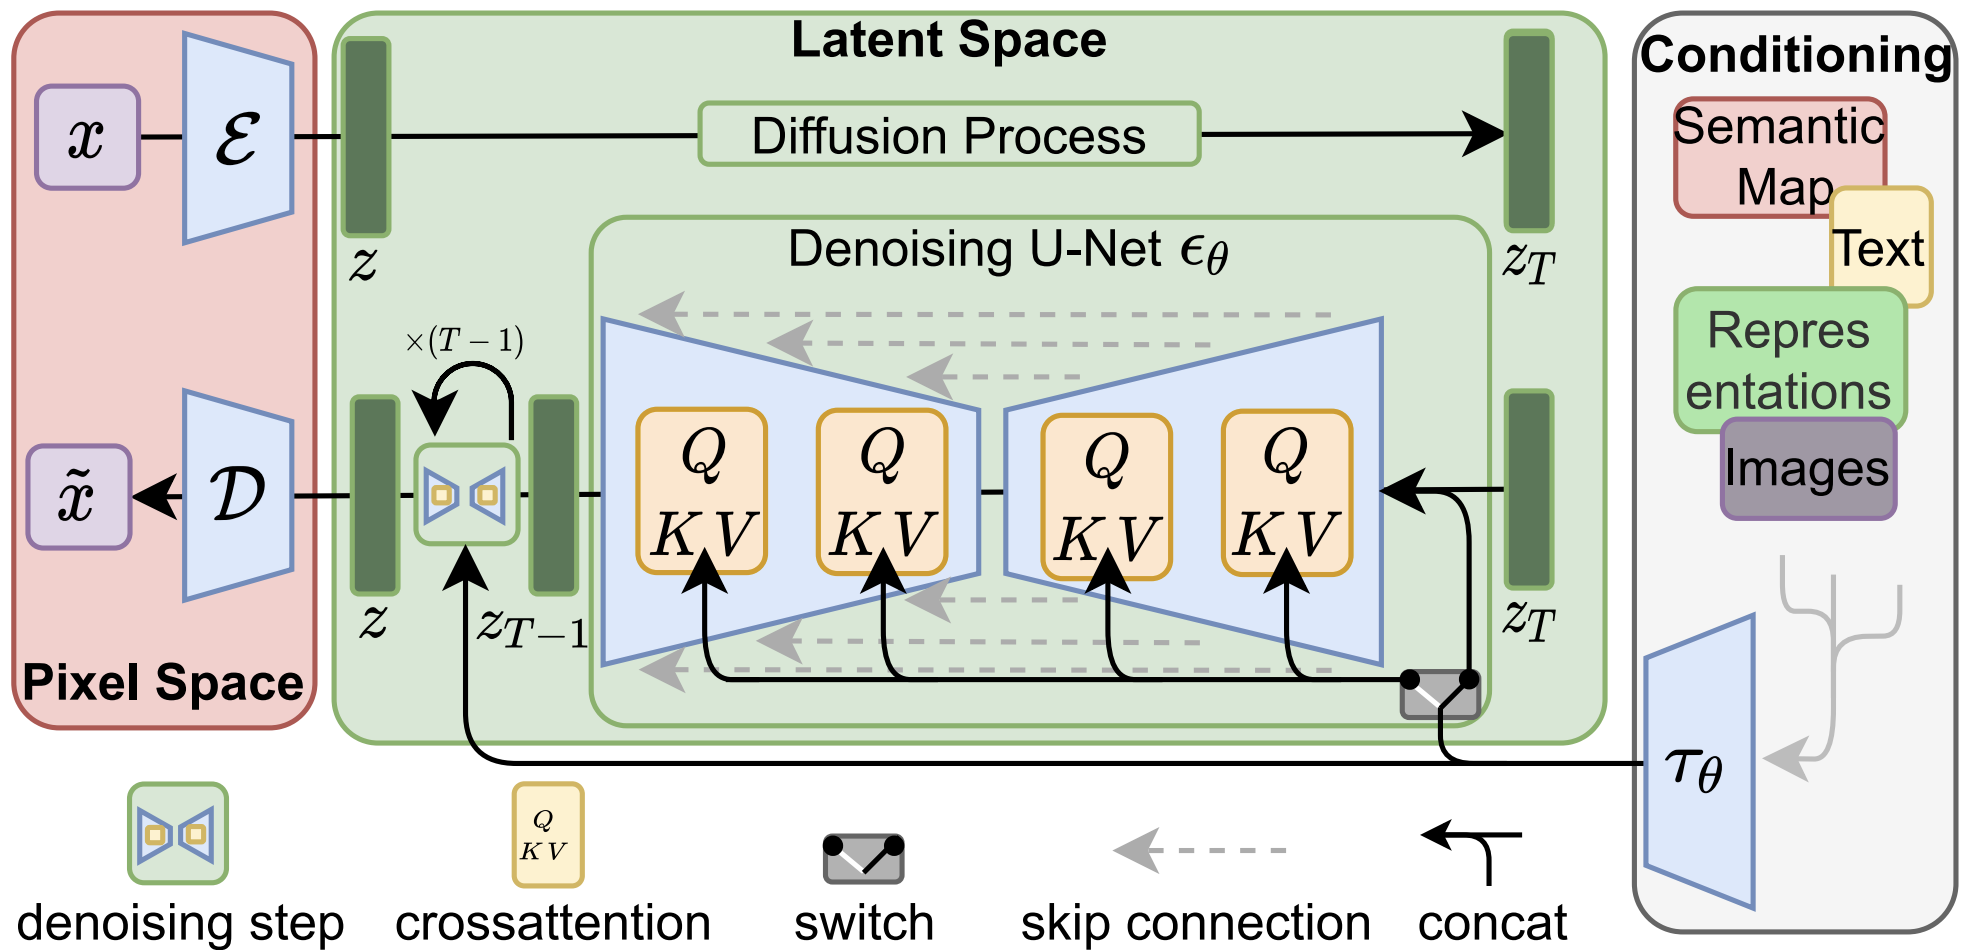
\includegraphics[width=0.8\textwidth]{images/diffusion_models/stable_diffusion/stable_diffusion.png}
    \caption{Stable diffusion scales better compared to other models \cite{stable_diffusion} (DALL-E, VQGAN) with less downsampling blocks (4 instead of 16 as needed by VQGAN).}
\end{figure}


Stable diffusion models are based on latent diffusion. In the paper \cite{stable_diffusion} the authors suggested that computing gradients directly on the pixel space is inefficient, since this space is high-dimentional and includes imperceptible details (high-frequency undesired details). Instead, they suggest to first convert the training images to a lower-dimensional latent space and then apply the diffusion processes on this space. The computation is done on the latent space instead of the pixel space. The authors showed that this approach scales better to higher dimension inputs, and showed significant competitive performance on multiple tasks while lowering significantly computational costs.  And finally, the authors introduced general purpose conditioning mechanism based on cross-attention which allows multi-modal training.

% This process is much more efficient, and in the paper \cite{stable_diffusion} the authors showed that the model can be trained on a single GPU with 16GB of memory. The model is trained on a 256x256 resolution CelebA-HQ dataset with 30 diffusion steps.

% An example of this is when giving an image to a person and asking them to describe the image, they will not describe the individual pixel values, but instead describe the high-level features of the image first.

A 2021 paper released by OpenAI \cite{openai_diffusion_beats_gans} shows that diffusion models can outperform GANs in terms of image fidelity by trading off diversity.














\subsection{U-Net backbone}

U-Net (first introduced in 2015) \cite{unet} is a convolutional neural network architecture that is commonly used in diffusion models, particularly in stable diffusion models and its variants. U-Net is used as a backbone for denoising the latent representations. The U-Net architecture is a symmetric encoder-decoder network with skip connections between the encoder and decoder. The skip connections help the network to learn better, the downsampling process of the encoder removes abstract features in the data, and so skip connections allow the model to skip these downsampling blocks and preserve high-level features. In the original DDPM paper \cite{ddpm} the authors didn't explicitly used U-Net, however they used CNN with residual blocks, which is similar in structure and intent to U-Net. 

\begin{figure}
    \centering
    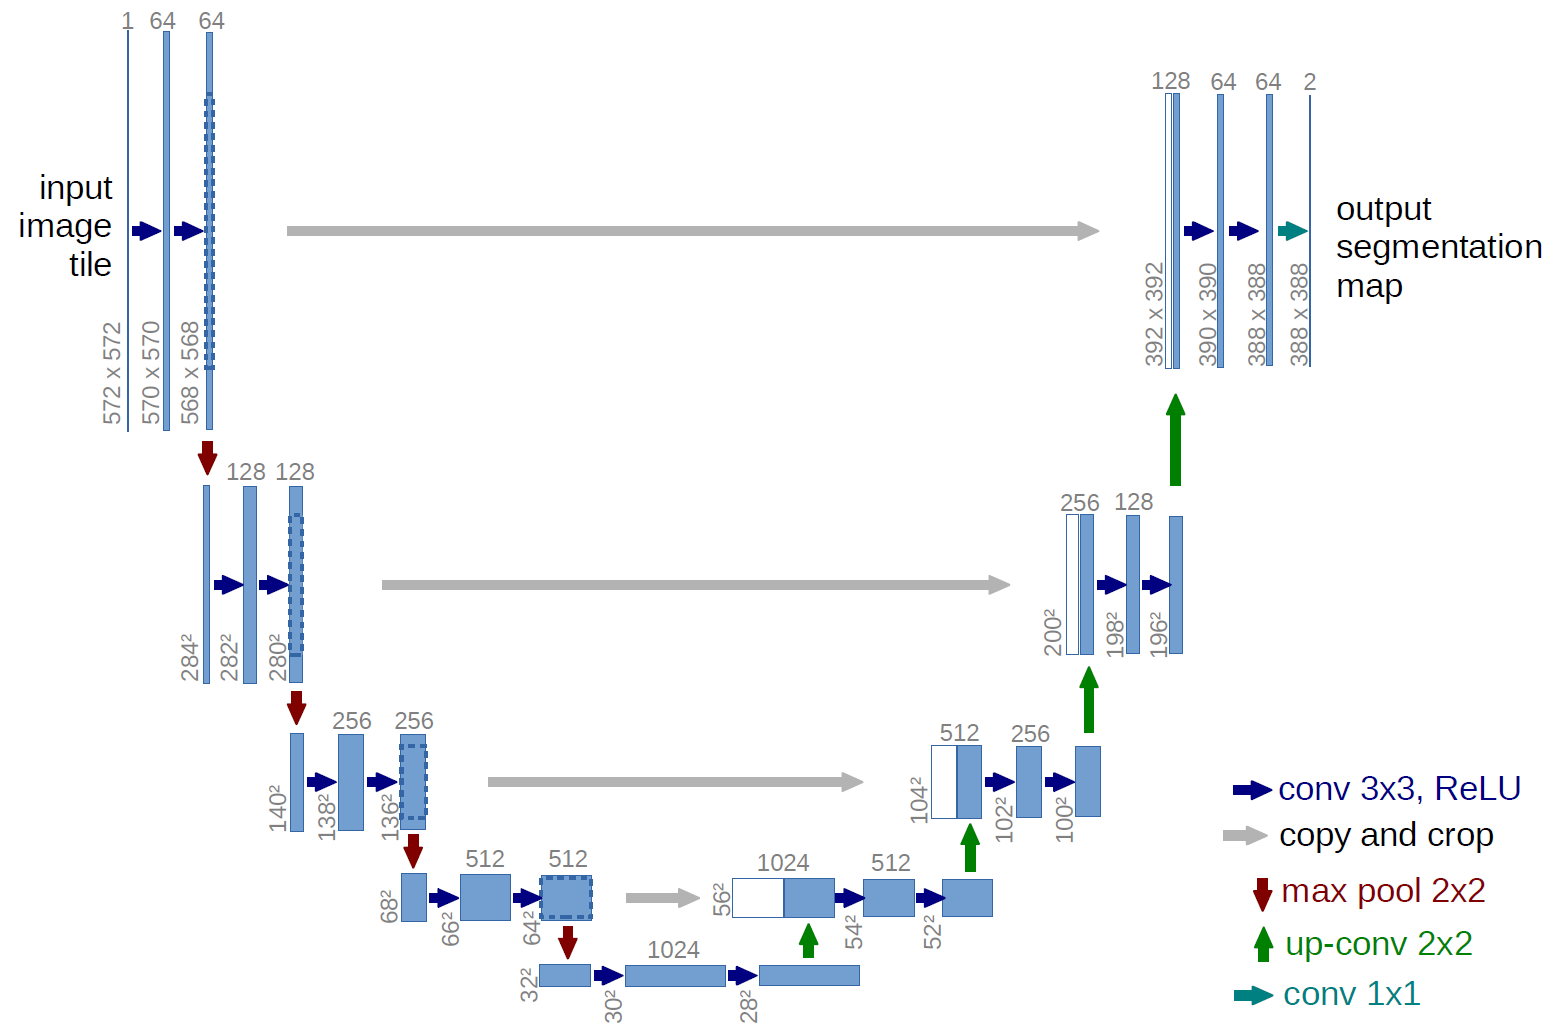
\includegraphics[width=0.8\textwidth]{images/diffusion_models/stable_diffusion/u-net-architecture.png}
    \caption{U-Net architecture \cite{unet}, with convolutional and deconvolutional layers, and skip connections. This architecture is commonly used in stable diffusion models.}
    \label{fig:unet_architecture}
\end{figure}

In figure \ref{fig:unet_architecture} the U-Net is shaped like a 'U' - notice that the layers downsample the input one after the other. Then, after we get to the desired depth, we start upsampling the input until we get output with the same dimensions as the input. The blue arrows are the convolutional layers with kernel size 3x3 and ReLU activation function. The max-pooling are the downsampling layers, and the upsampling layers are the deconvolutional layers.







\subsection{Architecture}

The stable diffusion model, which is a latent diffusion model, consists of: variational autoencoder which compresses the input images into regularized latent space, a U-Net backbone which denoises the output from forward diffusion backwards to obtain a latent representation, a variational autoencoder decoder which converts the latent representation back to the image space, and an optional classifier-free guidance mechanism which allows the model to be conditioned on text prompts or other images, which is domain-specific encoder. The high level architecture is shown in figure \ref{fig:stable_diffusion_architecture}.

\begin{figure}
    \centering
    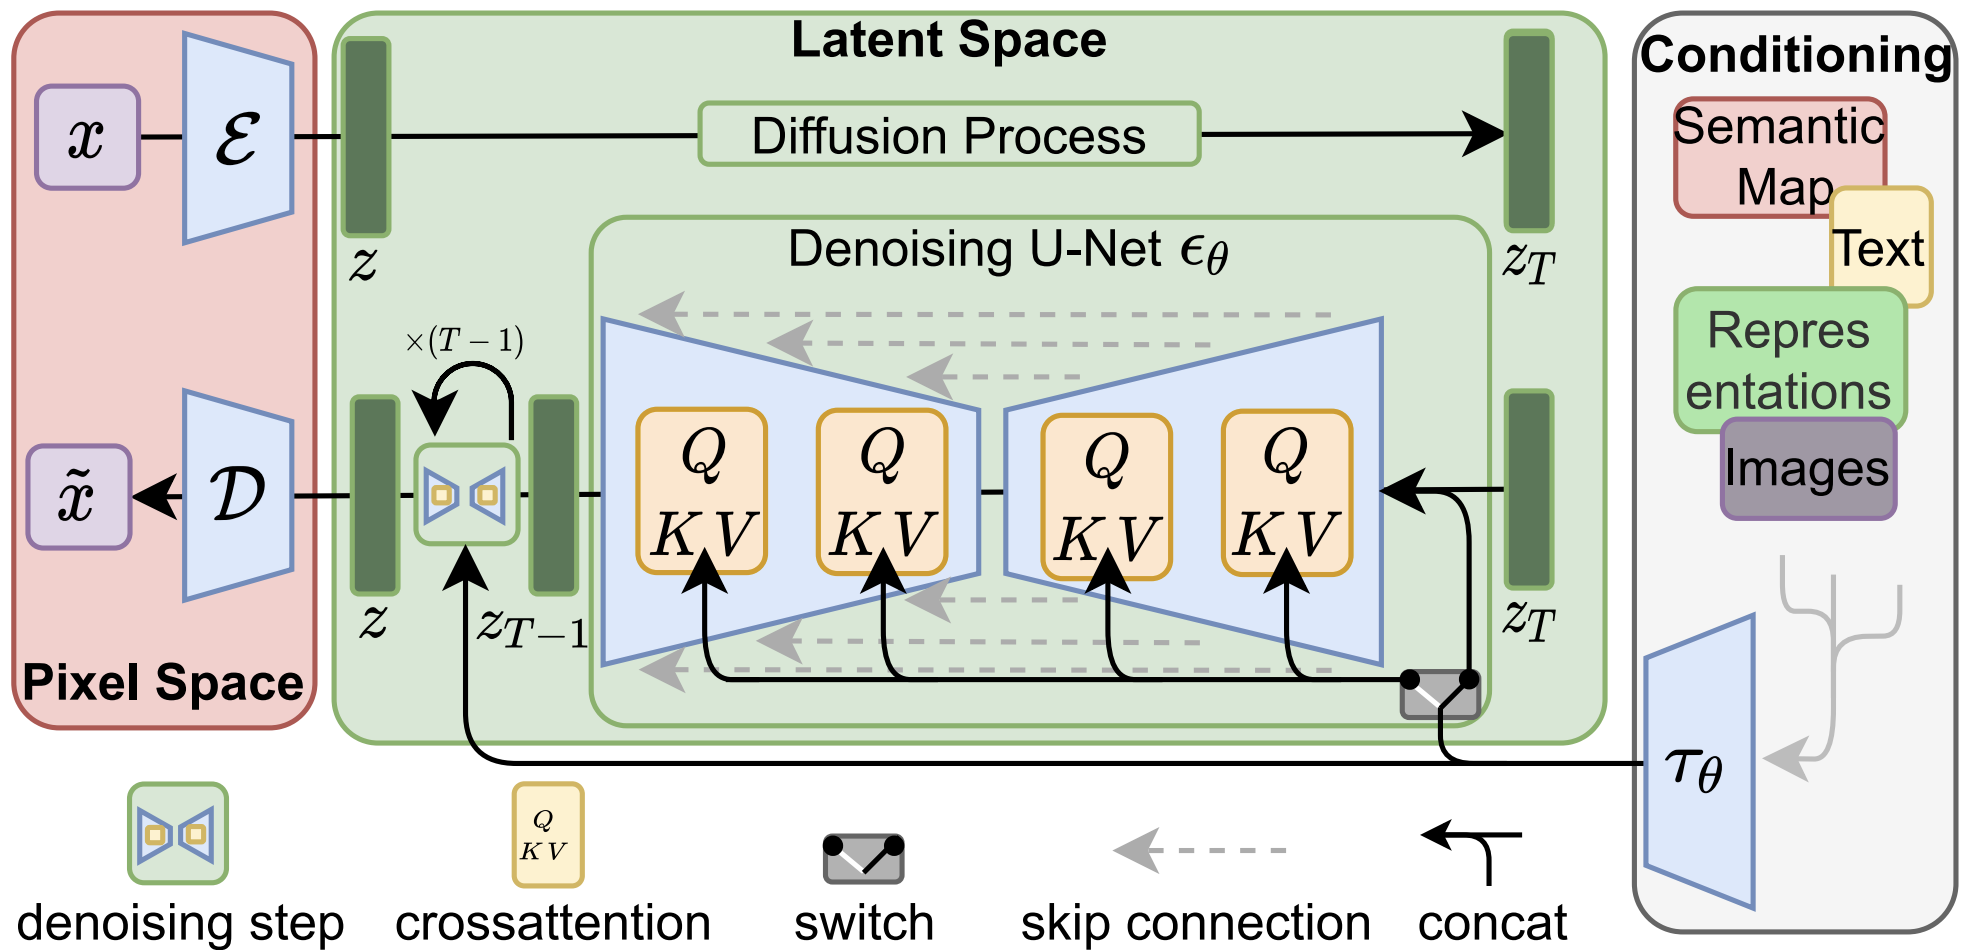
\includegraphics[width=0.75\textwidth]{images/diffusion_models/stable_diffusion/architecture.png}
    \caption{Stable diffusion architecture \cite{stable_diffusion}.}
    \label{fig:stable_diffusion_architecture}
\end{figure}

How the model is able to denoise latent space but also consider the conditional information? The authors used \textbf{cross-attention} mechanism. The cross-attention which was introduced in the transformers paper \cite{transformer}, is a mechanism that allows the model to focus on different parts of the input sequence. In the stable diffusion model, the cross-attention mechanism is used to focus on the latent space and the conditioning signal (text prompt or another image). 








\subsection{Classifier-free diffusion guidance}

\label{subsec:classifier_free_diffusion_guidance}

Conditioning a generative model can be achieved through various methods. How can we let our model understand our text prompt? Or condition on another image? One way is to train a model to learn a joint distribution of the training data and the conditioning signal $p(x,c)$ and then sample from the joint distribution. This, however, requires the training of a model for each separate conditioning signal.

Another approach is called \textbf{classifier guidance} \cite{openai_diffusion_beats_gans} which involves the training of a separate model to condition the output. The latest and most successful approach is called \textbf{classifier-free guidance} \cite{classifier_free_guidance}, in which, instead of training two networks, one conditional network and an unconditional network, we train a single network and during training, with some probability, we set the conditioning signal to zero. This way the network becomes a mix of conditioned and unconditioned network, and we can take the conditioned and unconditioned output and combine them with weight that indicates how much we want the network to pay attention to the conditioning signal. In other words, we control the weight of the conditioning signal during training 

To summorize, in contrast to classifier guidance, classifier-free guidance streamlines the training process and lowers computational costs by utilizing a single model instead of training two separate models.

\begin{lstlisting}[language=Python, caption={Classifier-free guidance (CFG) in Stable Diffusion. The CFG scale is the weight of the conditioning signal.}, label={lst:cfg_stable_diffusion}]
if do_cfg:
    output_cond, output_uncond = model_output.chunk(2)
    model_output = cfg_scale * (output_cond - output_uncond) + output_uncond
\end{lstlisting}

In listing \ref{lst:cfg_stable_diffusion} the code snippet is taken from \href{https://github.com/hkproj/pytorch-stable-diffusion/blob/e0cb06de011787cdf13eed7b4287ad8410491149/sd/pipeline.py#L131C1-L132C1}{a re-implementation of Stable Diffusion}, but the official implementation of Stable Diffusion is \href{https://github.com/CompVis/stable-diffusion/blob/21f890f9da3cfbeaba8e2ac3c425ee9e998d5229/ldm/models/diffusion/ddim.py#L178C1-L179C1}{very similar}.








\subsection{Contrastive Language Image Pre-training (CLIP)}

\label{subsec:clip}

In Stable Diffusion, the authors used CLIP as the text encoder for the conditional information of text prompts.

CLIP (Contrastive Language Image Pre-training) \cite{openai_clip} is a model developed by OpenAI that learns visual concepts from text supervision. The model builds associations between images and text prompts. 

This is why the researchers use the \textbf{CLIPTokenizer} which is part of the CLIP model. This tokenizer converts text prompts to a sequence of tokens which are then used in the latent space of the stable diffusion model. They use the embeddings of this pre-trained model.

\begin{figure}
    \centering
    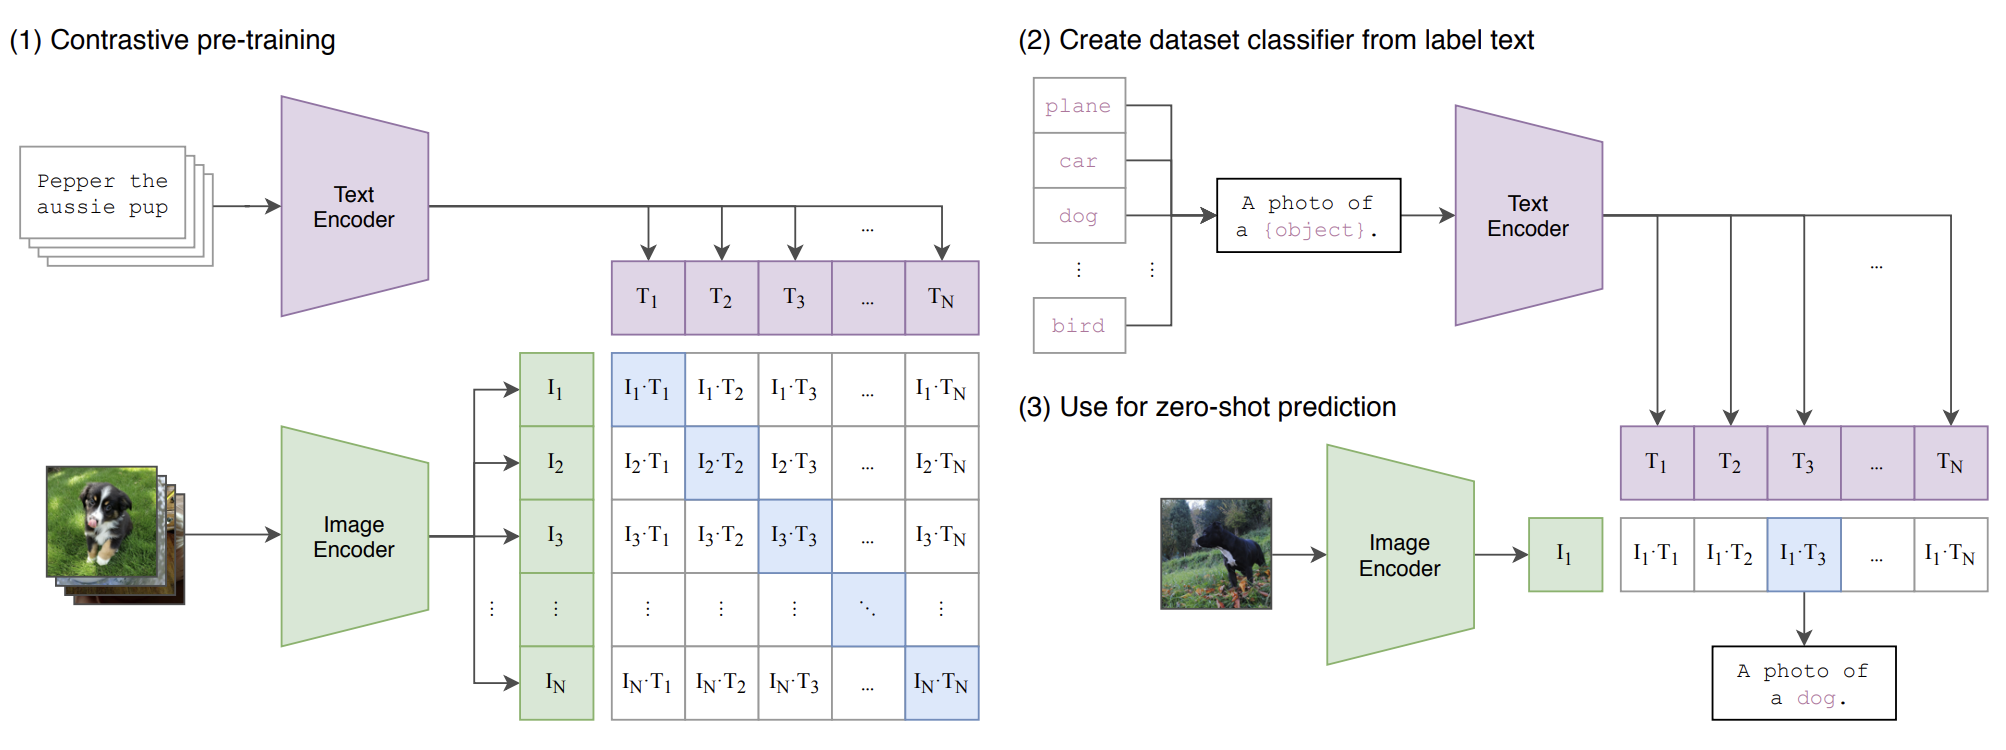
\includegraphics[width=1\textwidth]{images/diffusion_models/stable_diffusion/clip.png}
    \caption{(1) Contrastive pre-training stage of a CLIP model \cite{openai_clip} (training stage). The $I_1, ..., I_N$ are the images, and $T_1, ..., T_N$ are the text prompts. The output is a matrix of similarity scores between the images and the text prompts. (2) and (3) after the model is pre-trained its used as a zero-shot image classifier (the model can classify images without needing to be explicitly trained on specific classes).}
    \label{fig:openai_clip}
\end{figure}

In figure \ref{fig:openai_clip}, the diagonal of the similarity matrix ideally contains the highest scores for matching image-text pairs (idealy '1'), while the off-diagonal entries should have lower similarity scores (idealy '0'), indicating mismatches between images and texts.

The network implementation of CLIP is made up of an image encoder, which is typically a vision transformer (ViT) \cite{vision_transformer} or sometimes less commonly a ResNet \cite{resnet} model, while the text encoder is a text transformer \cite{transformer} or continous bag of words \cite{cbow_word2vec} (more commonly known as Word2Vec model by Google, 2013).

The CLIP model is trained using a contrastive objective, where the goal is to minimize the cosine distance between embeddings of matching image-text pairs (diagonal) and maximize the distance for non-matching pairs (off diagonal).






\subsection{Cross-attention}

Cross-attention is used in Stable Diffusion for multi-modal conditioning, it guides the model to output images based on conditional information. Although this information can be multi-modal (images, text, segmentation masks), the cross-attention mechanism is able to deal with them all.

Cross-attention, introduced in the Transformer paper \cite{transformer}, allows one set of inputs (query vectors) to attend (focus) on another set of inputs (the key vectors) and extract information from it. This is particularly useful in tasks where we want to condition one type of data on another, such as in image-text models (e.g. Stable Diffusion) where text guides the generation of images.

To understand cross-attention lets first understand \textbf{self-attention}:

In self-attention, the same set of data elements provides the queries, keys, and values. The mechanism computes attention scores based on how each element in the input interacts with other elements in the same sequence. This is widely used in transformers to capture relationships between tokens in a sequence. The formula for self-attention is given in the transformer paper \cite{transformer}.

\begin{equation}
    \text{Attention}(Q, K, V) = \text{softmax} \left( \frac{QK^T}{\sqrt{d_k}} \right) V
    \label{eq:self_attention}
\end{equation}

In equation \ref{eq:self_attention} we first do a cross-product of $Q$ and $K$ matrices, this gives us a matrix of attention scores for each pair of query vector and the key vector. We then divide the matrix by the square root of the dimension of the key vectors, this operation is done to normalize the large magnitude of the dot product, which stabilizes the gradients and the training. We then apply the softmax function, which converts the vector to a probability distribution between 0 and 1, which gives probability to tokens in the sequence. Finally, we multiply (dot product) the softmax output with the value vectors, which gives us the output of the self-attention.

\textbf{Cross-attention} is based on multiple self-attention heads (or blocks), and the input ($K$, $Q$, $V$) derive from the same input sequence. Cross-attention in comparison, each matrix comes from different source of sequence. For example, $Q$ could be an image embeddings (the VAE image encoder of stable diffusion), and $K$ and $V$ could represent a text prompt which gives attention to the image. This is the reason the researchers used cross-attention and not self-attention in the stable diffusion model, because of the multi-modal conditioning.

\begin{equation}
    \begin{aligned}
        \text{head}_i = \text{Attention}(QW_i^Q, KW_i^K, VW_i^V)  \\
        \text{MultiHead}(Q, K, V) = \text{Concat}(\text{head}_1, ..., \text{head}_h)W^O
    \end{aligned}
    \label{eq:cross_attention}
\end{equation}

Formula \ref{eq:cross_attention} describes a single self-attention head. Cross-attention is a concatenation of multiple self-attention heads, each with its own set of weights $W_i^Q$, $W_i^K$, $W_i^V$. The output of the cross-attention is the concatenation of the outputs of each head, and dot product with the output weights matrix $W^O$.



\begin{lstlisting}[language=Python, caption={Cross-attention PyTorch code snippet. The '@' operation is a dot product.}, label={lst:cross_attention_stable_diffusion}]
class CrossAttention(nn.Module):
def __init__(self, n_heads, d_embed, d_cross, 
        in_proj_bias=True, out_proj_bias=True):

    super().__init__()
    self.q_proj   = nn.Linear(d_embed, d_embed, bias=in_proj_bias)
    self.k_proj   = nn.Linear(d_cross, d_embed, bias=in_proj_bias)
    self.v_proj   = nn.Linear(d_cross, d_embed, bias=in_proj_bias)
    self.out_proj = nn.Linear(d_embed, d_embed, bias=out_proj_bias)
    self.n_heads = n_heads
    self.d_head = d_embed // n_heads

def forward(self, x, y):
    # ...

    weight = q @ k.transpose(-1, -2)
    weight /= math.sqrt(self.d_head)
    weight = F.softmax(weight, dim=-1)
    output = weight @ v

    output = output.transpose(1, 2).contiguous()
    output = output.view(input_shape)
    output = self.out_proj(output)
    return output
\end{lstlisting}

In listing \ref{lst:cross_attention_stable_diffusion} the code snippet is taken from \href{https://github.com/hkproj/pytorch-stable-diffusion/blob/e0cb06de011787cdf13eed7b4287ad8410491149/sd/attention.py#L100C1-L110C28}{a re-implementation of Stable Diffusion}, the official implementation of Stable Diffusion has \href{https://github.com/CompVis/stable-diffusion/blob/21f890f9da3cfbeaba8e2ac3c425ee9e998d5229/ldm/modules/attention.py#L152}{very complex cross-attention code}.











\subsection{DDIM Sampler}

\begin{figure}
    \centering
    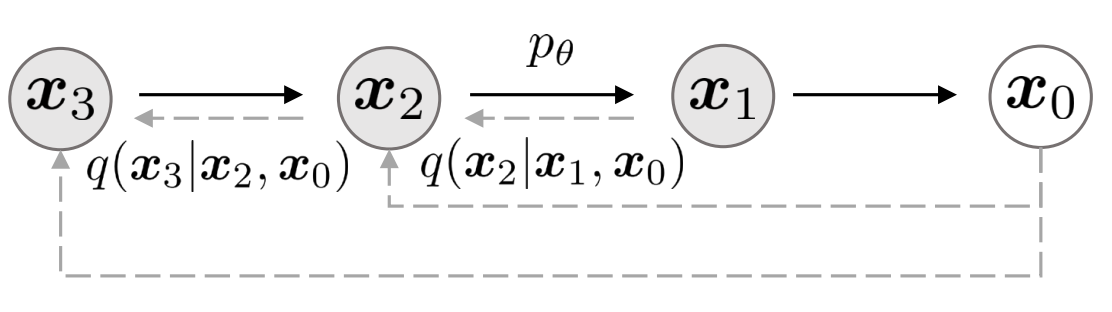
\includegraphics[width=0.8\textwidth]{images/diffusion_models/stable_diffusion/ddim_non_markov_process.png}
    \caption{Non-markovian inference model \cite{ddim} (denoising diffusion implicit models (DDIM) sampler). Each step not only depends on the previous step, but also on the initial step $x_0$.}
    \label{fig:ddim_non_markov_process}
\end{figure}

DDIM (Denoising Diffusion Implicit Models) (intoduced in a 2020 paper by Stanford) \cite{ddim} is a sampling method for diffusion models that offers improvements over the traditional DDPM (Denoising Diffusion Probabilistic Models) \cite{ddpm} approach. Unlike DDPM, which relies on a fixed noise schedule, DDIM introduces a more flexible noise schedule that allows for varying degrees of noise at different diffusion steps. This flexibility can lead to higher-quality and more diverse generated samples. Additionally, DDIM employs a more efficient sampling process, which can result in faster inference times and potentially better results.

In DDPM, images are generated by starting from pure noise and denoising it step-by-step through a Markovian chain (appendix \ref{appendix:markov_chains}). Each step adds a bit of noise to maintain probabilistic reversibility. This process is slow (10x to 50x times slower \cite{ddim}) and often requires hundreds to thousands (1000 steps in the case of Stable Diffusion \cite{stable_diffusion}) of denoising steps to generate a high-quality image. DDIM modifies the denoising process by introducing a \textbf{non-Markovian deterministic sampler} (figure \ref{fig:ddim_non_markov_process}). Instead of stochastically adding noise at each step, DDIM removes noise in a direct and controlled manner, skipping unnecessary steps and resulting in a deterministic path through the latent space.

In DDIM, the reverse process (denoising) can be viewed as solving an ordinary differential equation (ODE) in the latent space. DDIM simplifies the reverse process by computing intermediate noise-free latent variables without adding extra randomness.

To achieve this the researchers introduced a new family of forward process:

\begin{equation*}
    q_\sigma (x_{t-1} | x_t, x_0) = \mathcal{N} (\sqrt{\alpha_{t-1}} x_0 + \sqrt{1 - \alpha_{t-1} - \sigma_t^2} \cdot \frac{x_t - \sqrt{\alpha_t} x_0}{\sqrt{1 - \alpha_t}}, \sigma_t^2 I)
\end{equation*}

where $\sigma$ is a vector of indexes (of the steps): $\sigma \in \mathbb{R}^T_{\geq 0}$. The magnitude of $\sigma$ controls how stochastic the forward process is; when $\sigma \rightarrow 0$, we reach an extreme case where as long as we observe $x_0$ and $x_t$ for some $t$, then $x_{t-1}$ become known and fixed.

The distribution of $x_t$ is defined given $x_{t-1}$ and $x_0$ - the process is not longer markovian (this equation is derived from Bayes' rule, its also proven that this is also Gaussian distribution):

\begin{equation*}
    q_\sigma (x_t | x_{t-1}, x_0) = \frac{q_\sigma (x_{t-1} | x_t, x_0) q_\sigma (x_t | x_0)}{q_\sigma (x_{t-1} | x_0)}
\end{equation*}

Now in order to adapt to the reverse diffusion process (which is the entire goal of this paper, to skip intermediate steps of the sampling process), we define this process on the subset $\{ x_{\tau_1}, ..., x_{\tau_S} \}$:

\begin{equation}
    p_\theta (x_{0:T}) := p_\theta (x_T) \prod_{i=1}^{S} p_\theta^{(\tau_i)} (x_{\tau_{i-1}} | x_{\tau_i}) \times \prod_{t \in \bar{\tau}} p_\theta^{(t)} (x_0 | x_t)
    \label{eq:ddim_reverse_diffusion}
\end{equation}

\begin{figure}
    \centering
    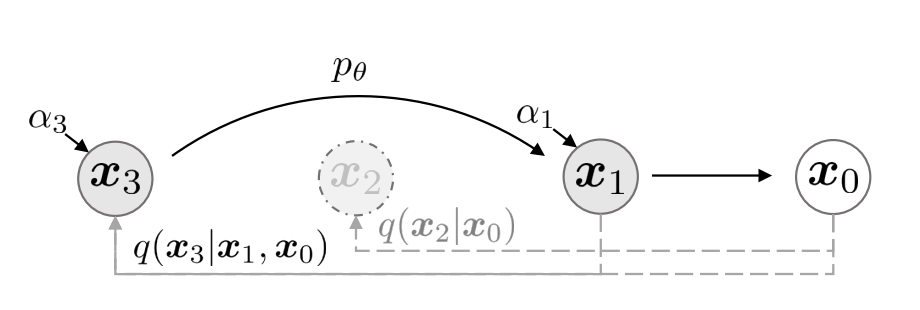
\includegraphics[width=0.8\textwidth]{images/diffusion_models/stable_diffusion/ddim_sampling_process.png}
    \caption{Reverse diffusion process of the DDIM sampler \cite{ddim} for accelerated generation of images. Here we see that $x_3$ depends only on $x_1$ (and not $x_2$) and $x_0$. This process can be generalized to all subsets of steps (eq. \ref{eq:ddim_reverse_diffusion}).}
    \label{fig:ddim_sampling_process}
\end{figure}

\begin{figure}
    \centering
    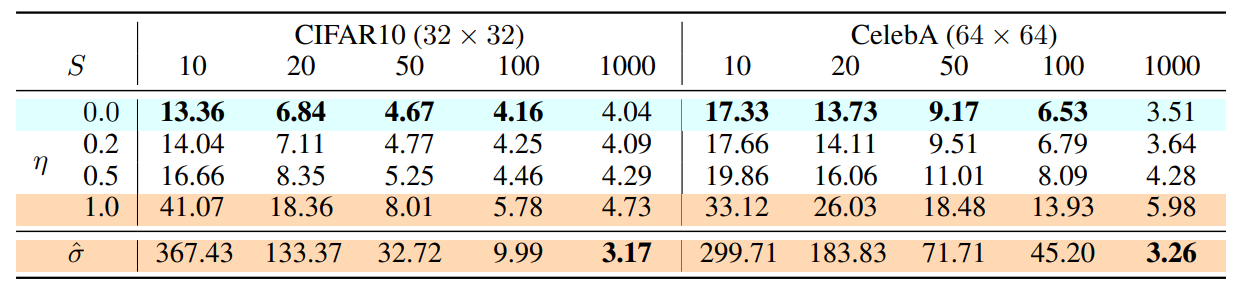
\includegraphics[width=0.8\textwidth]{images/diffusion_models/stable_diffusion/ddim_sample_quality.png}
    \caption{The researchers showed that using this non-Markovian process gives almost the same sample quality (in FID metric eq. \ref{eq:fid_score}, lower is better) as regular DDPM but much less computational cost (since we skip all the latent steps). In the figure, the researchers conducted experiments on CIFAR10 and CelebA datasets, with 10,20,50,100,1000 steps. The stochasticity of the model is controlled by $\eta$. When $\eta = 0$ (blue) the model is deterministic (DDIM process), and when $\eta = 1$ (orange) the model is stochastic (DDPM process).}
\end{figure}











\subsection{Training}

Stable diffusion uses two-stage approach, called classifier-free guidance (see \ref{subsec:classifier_free_diffusion_guidance}) which was discuessed before. In the paper the authors made simplified loss objective:

\[
    L_{\text{DM}} = \mathbb{E}_{x, \epsilon \sim \mathcal{N} (0, 1), t} [ \Vert \epsilon - \epsilon_\theta(x_t, t) \Vert _2^2 ]
\]